\documentclass[11pt,a4paper]{article}

\usepackage[utf8]{inputenc}
\usepackage[T1]{fontenc}
\usepackage[english]{babel}
\usepackage[margin=2.5cm]{geometry}
\usepackage{array}
\usepackage{hyperref}
\usepackage{plantuml}
\usepackage{graphicx}
\graphicspath{ {./images/} }

\title{EASNFW Requirements}
\author{}
\date{}

\begin{document}

\maketitle

\tableofcontents
\clearpage

% =============================================================================
\section{Introduction}
% =============================================================================

\subsection{Purpose}

The purpose of the software whose requirements are specified in this document
is to control the hardware of an ecoacoustic sensing node.

\subsection{Scope}

This document specifies the requirements for the software product designated
as EASNFW, from \textbf{e}co\textbf{a}coustic \textbf{s}ensing \textbf{n}ode
\textbf{f}irm\textbf{w}are.

Within this document, EASNFW may also be referred to as \textit{the firmware}.
The ecoacoustic sensing node as a whole, comprising all software and hardware
components of the device, is designated as EASN and may also be referred to as
\textit{the system} or \textit{the sensing node}.

The purpose of EASNFW is to control the hardware of EASN in order to:

\begin{itemize}
    \item acquire ecoacoustic data through the system sensors;
    \item process the acquired data; and
    \item transmit the acquired and processed data to a cloud platform.
\end{itemize}

The cloud platform may be referred to as \textit{the cloud platform} or simply
\textit{the cloud}. The acquired data is intended for use in ecoacoustic
studies.

\subsection{Product Overview}

\subsubsection{Product Perspective}

The system is intended to integrate a distributed ecoacoustic data acquisition
infrastructure. This infrastructure is composed of a set of sensing nodes and a
cloud platform.

The cloud platform stores the data acquired by the sensing nodes and provides
support for visualizing and analyzing the collected data.

The system hardware is based on the boards nRF5340 Audio DK and nRF9151 SMA DK
from Nordic Semiconductor.

EASNFW will run on and control the nRF5340 System-on-Chip (SoC) from the
nRF5340 Audio DK and the nRF9151 System-in-Package (SiP) from the nRF9151 SMA
DK. EASNFW is hence subdivided into two different components: one that will run
on nRF5340 and be mainly responsible for interfacing with the system sensors,
and processing, storing and retrieving the data acquired through them, and is
therefore designated as EASNFW-SENSOR; and another one that will run on nRF9151
and be mainly responsible for interfacing with the cloud, and is therefore
designated as EASNFW-CLOUD. EASNFW-SENSOR and EASNFW-CLOUD will communicate
over SPI, with EASNFW-SENSOR as the controller and EASNFW-CLOUD as the
peripheral.

The sensors with which EASNFW-SENSOR interfaces are described in Table
\ref{table:sensors}.

% TODO: confirm mic/audio sensor details
\begin{table}[h!]
\centering
\begin{tabular}{ m{4cm} m{3.5cm} m{6cm} }
    Sensor                                                   & Part Number                  & Connection \\
    \hline
    Audio (microphone)                                       & VM3011 (Vesper Technologies) & Connected to nRF5340 through I2C with address 0x60 \\
    Environmental (temperature, humidity, pressure and VOCs) & BME688 (Bosch)               & Connected to nRF5340 through I2C...
\end{tabular}
\caption{System sensors description}\label{table:sensors}
\end{table}

EASNFW-CLOUD will communicate with the cloud using HTTP over LTE-M through the
built-in LTE-M modem of nRF9151. Communication is unidirectional: data flows
from the sensing node to the cloud, but not from the cloud to the sensing node.

\paragraph{User interfaces}

EASNFW-SENSOR will provide a command line interface (CLI) for verifying
specific features. Such interface will only be enabled when working with the
``CLI verification image'' (see Section~\ref{sec:firmware-images}).

Both EASNFW-SENSOR and EASNFW-CLOUD will log its own activities through the
serial-USB interface of their respective boards when logging is enabled.

\subsubsection{Product Functions}

The main functions that will be performed by EASNFW are described in Table
\ref{table:easnfw-functions}, alongside the firmware component responsible for
each function.

\begin{table}[h!]
\centering
\begin{tabular}{ m{6cm} m{6cm} }
    Function                                                                   & Responsible firmware component \\
    \hline
    Acquire audio data                                                         & EASNFW-SENSOR                 \\
    Process audio data                                                         & EASNFW-SENSOR                 \\
    Acquire environmental data                                                 & EASNFW-SENSOR                 \\
    Transmit acquired environmental data and processed audio data to the cloud & EASNFW-CLOUD
\end{tabular}
\caption{EASNFW functions description}\label{table:easnfw-functions}
\end{table}

\subsubsection{System architecture overview}

Figure \ref{fig:sysarchoverview} provides an overview of the system
architecture.

\begin{figure}[h!]
    \centering
    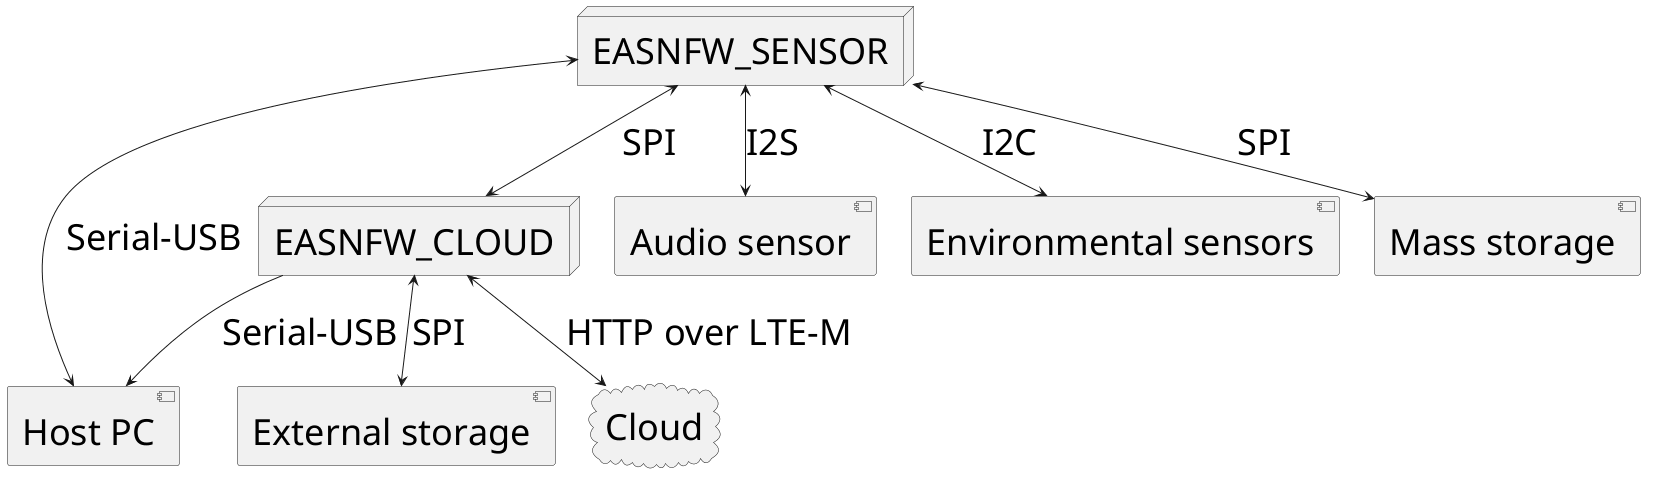
\includegraphics[width=1\textwidth]{sys_arch}
    \caption{System architecture overview}\label{fig:sysarchoverview}
\end{figure}

% TODO: instead of having the following paragraph and table, just add details
% about things from the above diagram since it's all the same. Or just have the
% table and then add details.

The main peripherals with which EASNFW will communicate are described in Table
\ref{table:peripherals}, alongside the firmware component responsible for
communicating with each peripheral and the communication protocol or technology
used.

% TODO: confirm mic/audio sensor details
\begin{table}[h!]
\centering
\begin{tabular}{ m{4.5cm} m{3.5cm} m{6cm} }
    Peripheral                                                              & Responsible firmware component & Communication protocol/technology \\
    \hline
    Audio sensor (VM3011)                                                   & EASNFW-SENSOR                  & I2S (audio data) \\
    Environmental sensor (BME688)                                           & EASNFW-SENSOR                  & I2C \\
    Mass storage (Built-in SD card holder from nRF5340 Audio DK SD)         & EASNFW-SENSOR                  & SPI \\
    External memory (Built-in flash memory from nRF9151 SMA DK)             & EASNFW-CLOUD                   & SPI
\end{tabular}
\caption{Peripherals description}\label{table:peripherals}
\end{table}

\subsubsection{User Characteristics}

Users of EASN and EASNFW are expected to be familiar with general concepts
related to:

\begin{itemize}
    \item embedded systems;
    \item Internet of Things (IoT);
    \item wireless communication; and
    \item digital signal processing (DSP).
\end{itemize}

\subsubsection{Limitations}

EASNFW functions and their implementations are constrained by:

\begin{itemize}
    \item the computational, memory, communication, and energy resources of the
          target hardware; and
    \item the interfaces provided by the cloud platform.
\end{itemize}

\subsection{Definitions}

\textbf{Audio track}

An ordered collection of audio samples captured sequentially over a continuous
period of PARAM\_TRACK\_LEN seconds, which will be configurable via Kconfig.

\textbf{Audio processing algorithm}

The algorithm used to process the recorded audio tracks.

\textbf{Processed audio track}

The output, or collection of outputs, produced by the audio processing
algorithm for a given audio track.

\textbf{Environmental sample set}

A set of environmental variables sampled within a short interval. The set
consists of temperature, humidity, pressure and VOCs.

\textbf{Self-test sequence}

Sequence of tests executed by EASNFW to verify the correct working of
individual software modules, as well as the integration between them. It is
broken down into the independent self-test sequence, which is firmware
component-specific sequence, meaning that each of EASNFW-SENSOR and
EASNFW-CLOUD has its own independent self-test sequence; and the shared
self-test sequence, which is carried out by EASNFW-SENSOR and EASNFW-CLOUD
together.

\textbf{Verification images}

Set of images intended to be used solely for verification, comprehends the
regression verification image and the CLI verification image (see
Section~\ref{sec:firmware-images}).

\subsection{Firmware Images}
\label{sec:firmware-images}

\textbf{Production image}

Image of the firmware to be used for deployment. Contains all the business
logic and logging is disabled. Built when the BUILD\_PROD flag is set.

\textbf{Debugging image}

Image of the firmware to be used for debugging, it is the same as the
production image but with logging enabled. Built when the BUILD\_DEBUG flag is
set.

\textbf{Development image}

Image of the firmware to be used for development, it is the same as the
debugging image, but with the self-test sequence included. Built when the
BUILD\_DEVELOP flag is set.

\textbf{Regression verification image}

Image of the firmware that contains only the self-test sequence with logging
enabled. Built when the BUILD\_REGR flag is set.

\textbf{CLI verification image}

Image of the firmware to be used for verifying specific product functions, such
as the audio acquisition and processing, through a command-line interface (CLI)
running on EASNFW-SENSOR. Built when the BUILD\_CLI flag is set. Only valid for
EASNFW-SENSOR.

\subsection{Payloads}

\textbf{Ecoacoustic data payload}

A payload transmitted periodically to the cloud that consists of a processed
audio track paired with an atmospheric sample set and a timestamp indicating
when the corresponding audio track was recorded.

\textbf{Power-on payload}

A payload transmitted to the cloud during EASNFW initialization that consists
of EASNFW-SENSOR and EASNFW-CLOUD respective revisions and the reason why the
device was last powered off.

% =============================================================================
\section{Architecture}
% =============================================================================
\label{sec:architecture}

EASNFW is based on the Zephyr RTOS and on the utilities provided by the nRF
Connect SDK. Each firmware component is composed of an initialization routine
and a set of threads that communicate with each other using message queues.
Hardware is driven through the Zephyr device drivers, which expose the
peripheral interrupts to the firmware.

\subsection{EASNFW-SENSOR}

EASNFW-SENSOR is composed of the following modules:

\begin{itemize}
    \item \textbf{sample audio}: controls the audio sampling process;
    \item \textbf{sample environmental data}: controls the environmental data
          sampling process;
    \item \textbf{I2S}: drives the I2S peripheral to acquire audio data from
          the audio sensor;
    \item \textbf{I2C}: drives the I2C peripheral to acquire environmental
          data from the environmental sensor and to configure the audio
          sensor;
    \item \textbf{SPIM}: drives the SPI peripheral in controller mode to
          control the mass storage and to send commands to and receive
          responses from EASNFW-CLOUD;
    \item \textbf{cloud}: handles, at a higher level, the communication with
          EASNFW-CLOUD;
    \item \textbf{audio processing}: processes the acquired audio tracks
          according to the audio processing algorithm;
    \item \textbf{mass storage}: reads from and writes to the mass storage;
    \item \textbf{nvs}: reads from and writes to the internal flash;
    \item \textbf{log}: controls the log behavior;
    \item \textbf{self-test}: executes the EASNFW-SENSOR self-test sequences;
    \item \textbf{cli}: provides the command line interface for verifying
          specific features;
    \item \textbf{power management}: manages the energy-saving states.
\end{itemize}

EASNFW-SENSOR runs at least two threads: a sensor sampling thread, which
samples the audio data through the I2S module and the environmental data
through the I2C module; and a cloud communication thread, which sends the data
to be transmitted to the cloud to EASNFW-CLOUD through the cloud and SPIM
modules. The I2S module is driven by an interrupt that is triggered when the
I2S RX buffer is full, indicating that a block of audio samples is ready to be
processed.

\begin{figure}[h!]
    \centering
    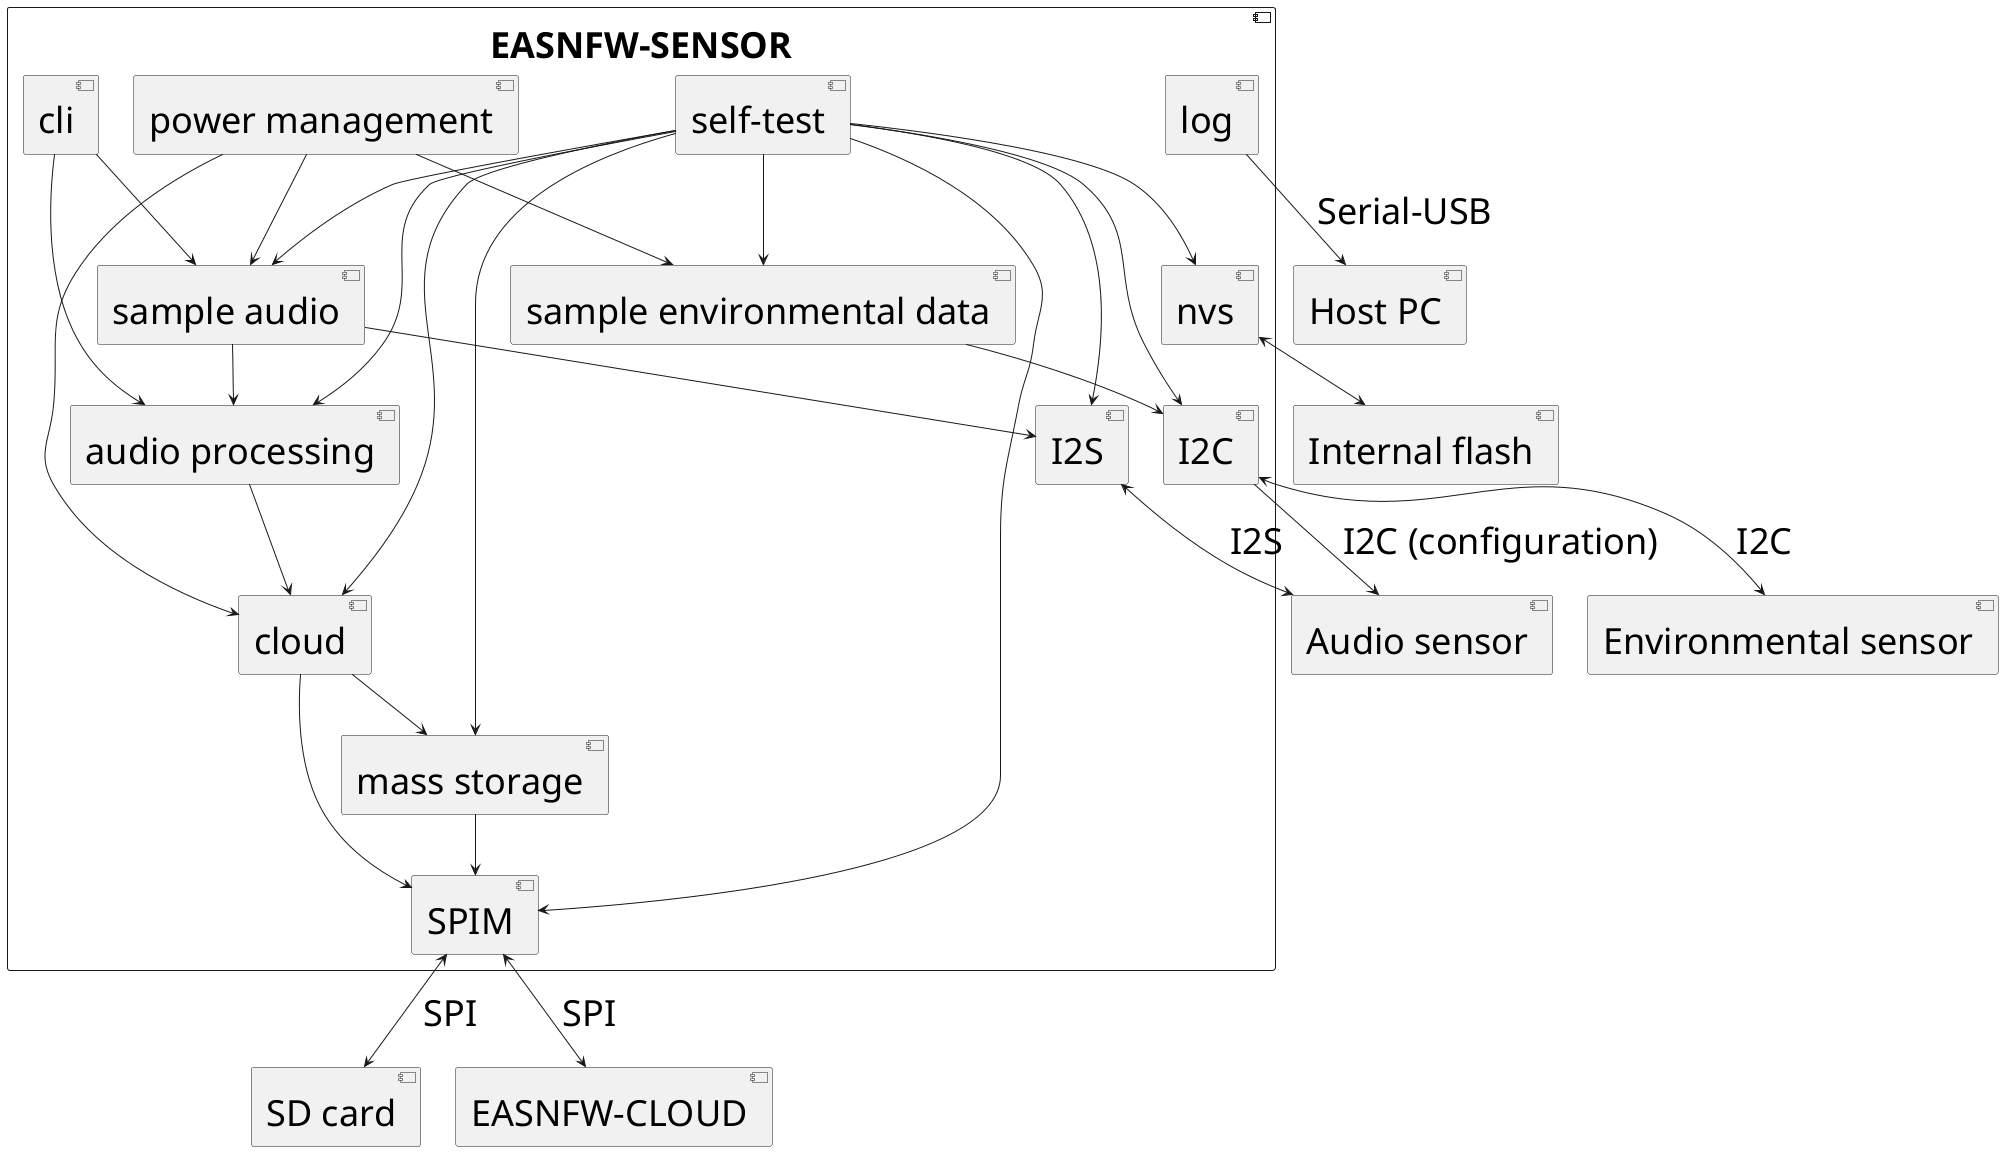
\includegraphics[width=1\textwidth]{easnfw_sensor_modules}
    \caption{EASNFW-SENSOR module diagram}\label{fig:easnfw-sensor-modules}
\end{figure}

The EASNFW-SENSOR module diagram is presented in Figure
\ref{fig:easnfw-sensor-modules}.

\subsection{EASNFW-CLOUD}

EASNFW-CLOUD is composed of the following modules:

\begin{itemize}
    \item \textbf{SPIS}: drives the SPI peripheral in peripheral mode to
          receive commands from and send responses to EASNFW-SENSOR;
    \item \textbf{EASNFW-SENSOR}: handles, at a higher level, the
          communication with EASNFW-SENSOR;
    \item \textbf{log}: controls the log behavior;
    \item \textbf{cloud}: handles the cloud transmission logic;
    \item \textbf{LTE-M}: handles the LTE-M specifics;
    \item \textbf{HTTP}: provides the HTTP client used to transmit payloads to
          the cloud;
    \item \textbf{external memory}: reads from and writes to the external
          storage;
    \item \textbf{SPIM}: drives the SPI peripheral in controller mode to
          control the external memory;
    \item \textbf{self-test}: executes the EASNFW-CLOUD self-test sequences;
    \item \textbf{power management}: manages the energy-saving states.
\end{itemize}

EASNFW-CLOUD runs at least two threads: a data reception thread, which receives
the data from EASNFW-SENSOR through the SPIS and EASNFW-SENSOR modules; and a
cloud transmission thread, which sends the payloads to the cloud through the
cloud, HTTP and LTE-M modules. EASNFW-CLOUD is driven by interrupt sources such
as the SPIS receive events, which indicate that data has been received from
EASNFW-SENSOR, and the LTE-M events, which indicate changes in the state of the
LTE-M modem.

The EASNFW-CLOUD module diagram is presented in Figure
\ref{fig:easnfw-cloud-modules}.

\begin{figure}[h!]
    \centering
    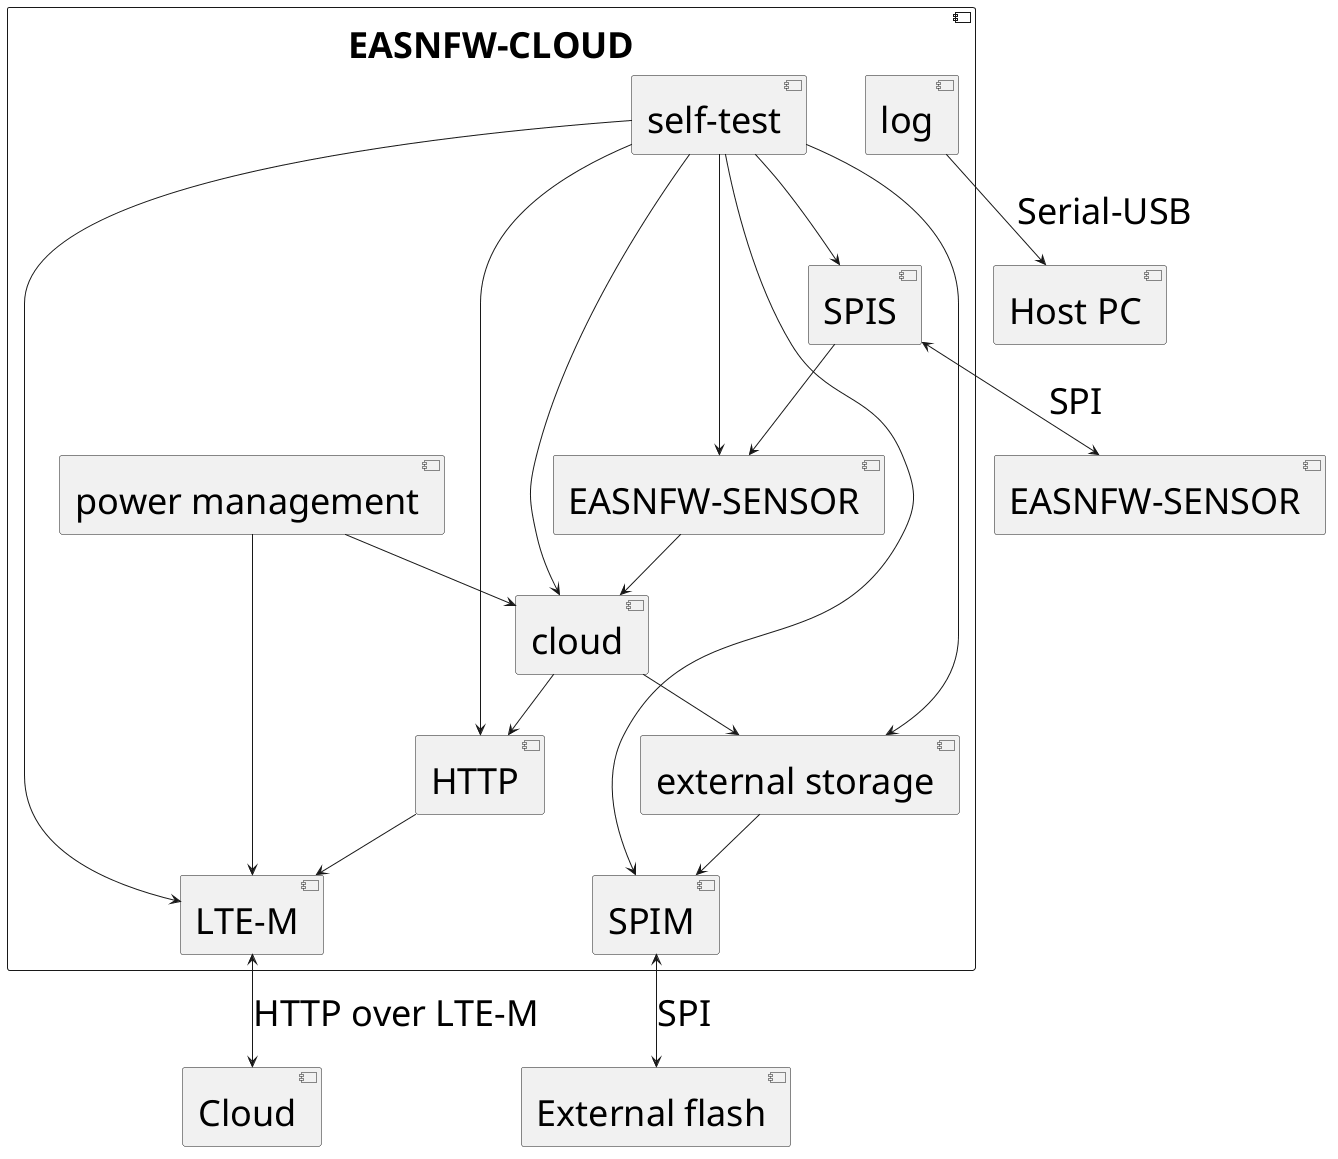
\includegraphics[width=1\textwidth]{easnfw_cloud_modules}
    \caption{EASNFW-CLOUD module diagram}\label{fig:easnfw-cloud-modules}
\end{figure}

% =============================================================================
\section{Requirements}
% =============================================================================

\subsection{Initialization}

\subsubsection{REQ-001}

When the system is powered on, the firmware shall execute the initialization
sequence, which comprehends: (a) initializing critical peripherals\footnote{(a)
is already taken care of by Zephyr.}; (b) running the self-test
sequences\footnote{(b) is only valid for the firmware images that include the
self-test sequences.}; (c) stablishing an Internet connection; (d) transmitting
the power-on payload to the cloud; and (e) transmitting to the cloud any
pending ecoacoustic data payloads from previous boot cycles.

\subsubsection{REQ-002}

After the initialization sequence is successfully completed, the firmware shall
periodically sample the audio into PARAM\_TRACK\_LEN-second audio tracks with a
PARAM\_INTER\_TRACK\_INTERVAL-second interval between the sampling of two
consecutive audio tracks.

Parameters for audio sampling:

\begin{itemize}
    \item Number of channels: 1
    \item Sample rate: PARAM\_AUDIO\_SAMPLE\_RATE kHz
    \item Bandwidth: PARAM\_AUDIO\_SAMPLE\_BW\_LO Hz -
          PARAM\_AUDIO\_SAMPLE\_BW\_HI kHz
    \item Sample width: PARAM\_AUDIO\_SAMPLE\_WIDTH bits
\end{itemize}

\subsubsection{REQ-003}

The firmware shall process the audio tracks according to the audio processing
algorithm.

\subsubsection{REQ-004}

Before the beginning of the sampling of each audio track, the firmware shall
capture a timestamp and sample the environmental data.

\subsubsection{REQ-005}

After an audio track is processed, the firmware shall send the processed audio
track, alongside the timestamp and environmental data that were captured before
the beginning of the sampling of that audio track sampling, to the cloud.

\subsubsection{REQ-006}

When the transmission of the power-on payload to the cloud fails, the firmware
shall retry transmitting it up to PARAM\_NUM\_RETRY\_TX\_CLOUD times with an
exponential backoff model defined by $t[s]=2^c$, where $c$ is the number of
times that the transmission has been retried.

\subsubsection{REQ-007}

When the transmission of the power-on payload to the cloud fails, the firmware
shall retry transmitting it until the free space of the mass storage is
insufficient to store the data relative to another audio track. The firmware
shall use an exponential backoff model defined by $t[s]=2^c$, where $c$ is the
number of times that the transmission has been retried.

\subsubsection{REQ-008}

The firmware shall persist ecoacoustic data payloads that have not been sent to
the cloud using across boot cycles.

\subsubsection{REQ-009}

The firmware shall persist details of fatal failures across boot cycles.

\subsubsection{REQ-010}

When the firmware is waiting for triggers to take action, the firmware shall
enter an energy-saving state.

\subsubsection{REQ-011}

The following parameters shall be configurable at compile-time via Kconfig:

\begin{itemize}
    \item PARAM\_TRACK\_LEN (seconds)
    \item PARAM\_INTER\_TRACK\_INTERVAL (seconds)
    \item PARAM\_NUM\_RETRY\_TX\_CLOUD
    \item PARAM\_AUDIO\_SAMPLE\_RATE (kHz)
    \item PARAM\_AUDIO\_SAMPLE\_BW\_LO (Hz)
    \item PARAM\_AUDIO\_SAMPLE\_BW\_HI (kHz)
    \item PARAM\_AUDIO\_SAMPLE\_WIDTH (bits)
\end{itemize}

\subsubsection{REQ-012}

The firmware shall log information relevant to verifying correct system
operation and to identifying and diagnosing failures, in a way that the logs can
be monitored in real-time from a host personal computer (PC) through USB.

\subsubsection{REQ-013}

The firmware shall be designed so that communication parameters can be adapted
to the regulatory requirements of different geographical regions.

\end{document}